\documentclass[12pt]{article}

\usepackage{times}
\usepackage{textcomp}
\usepackage{listings}
\usepackage{fullpage}
\usepackage{color}
\usepackage{hyperref} 
\usepackage{pst-tree} 
\usepackage{verbatim} 
\usepackage{graphicx}
\usepackage{amsmath,amsfonts,amssymb,amsthm}
\graphicspath{ {./}}


\def\part#1{\item[\bf #1)]}
\renewcommand{\thesubsection}{Question \arabic{subsection}}

\author{Clement Tsang}

\begin{document}

\begin{center}
\Large\textbf{CS 241, Lecture 15 - Type Checking}
\textbf{Thurs, Mar 07, 2019}
\end{center}

\section{Warm Up Problem}
Consider the following grammar:
\begin{align*}
    &S' \rightarrow \vdash S \dashv \qquad (1)\\
    &S \rightarrow aS \qquad (2)\\
    &S \rightarrow B \qquad (3)\\
    &B \rightarrow aBb \qquad (4)\\
    &B \rightarrow \epsilon \qquad (5)
\end{align*}
Draw the SLR(1) transducer (and hence also an LR(0) transducer) for this grammar.  Is it LR(0)?  What about SLR(1)?

We see in the diagram that it is NOT LR(0), there are shift-reduce conflicts.  We remedy those by checking the Follow in states 2 and 8.

\section{Creating a Parse Tree}
Building the Parse Tree:
\begin{itemize}
    \item The difference between top-down parsing and bottom-up parsing is that in top-down, you pop a symbol $S$ from the stack and push the next rule, and make the new symbols the children of the popped symbol.  With bottom-up parsing, you reduce symbols into another rule, and keep the old symbols as the children.
    \item For example, for bottom-up, if we had the grammar:\\
        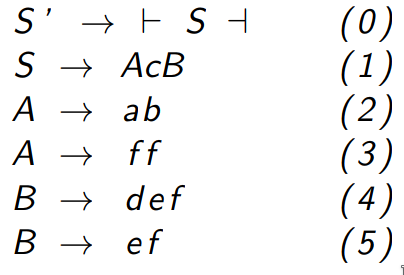
\includegraphics[scale=0.5]{bottom_up_grammar.png}\\
        Then for a string $\vdash abcdef \dashv$:\\
        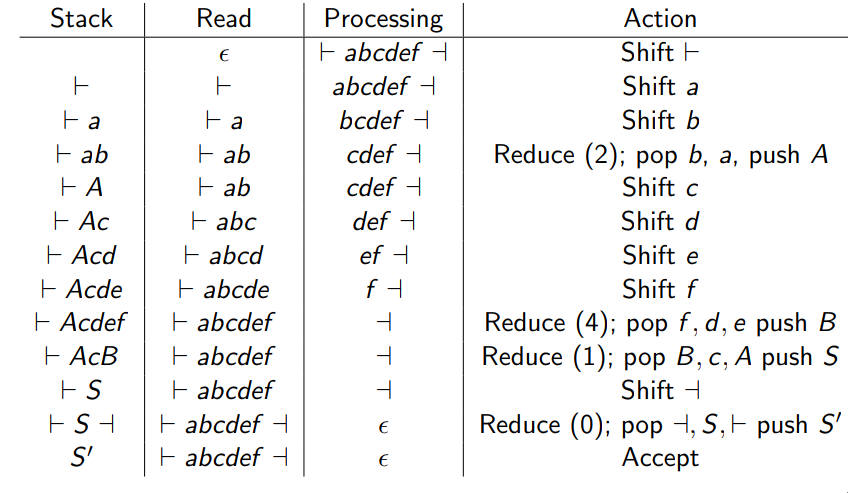
\includegraphics[scale=0.5]{bottom_up_table.png}\\
        We get the following parse tree:\\
        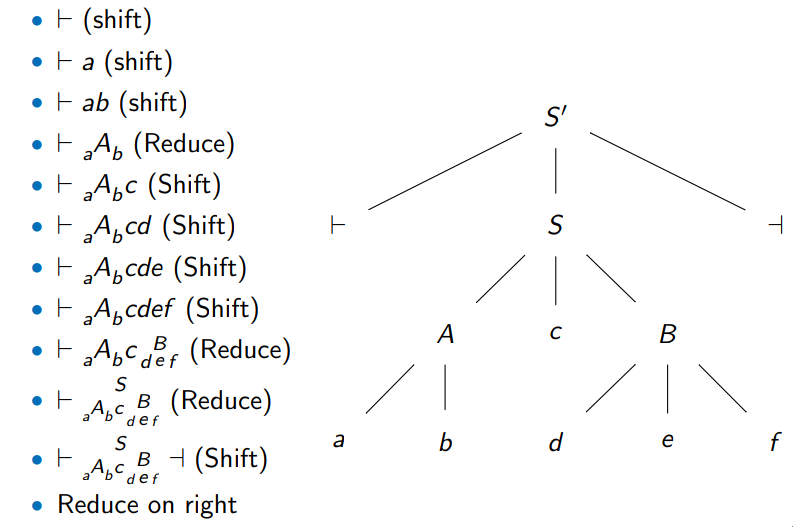
\includegraphics[scale=0.5]{bottom_up_parse_tree.png}
    \item We get this image for how grammars are classified:\\
        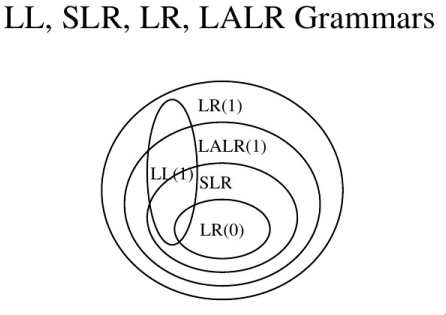
\includegraphics[scale=0.5]{grammar_pic.png}
\end{itemize}

\section{Parser and Assignment Information}
\begin{itemize}
    \item Our parser will output a .wlp4i file.  For example:
        \begin{align*}
            &S \rightarrow BOF e EOF \\
            &e \rightarrow e + t \\
            &e \rightarrow t \\
            &t \rightarrow ID
        \end{align*}
        with input $BOF a + b + c EOF$, where $a, b, c$ are IDs, then you will get the file:
        \begin{lstlisting}[mathescape, numbers=none, breaklines=true]
        S BOF e EOF
        BOF BOF
        e e + t
        e e + t
        e t
        t ID
        ID a
        + +
        t ID
        ID b
        + +
        t ID
        ID c
        EOF EOF
        \end{lstlisting}
    \item As an overview:
        \begin{itemize}
            \item A6 is WLP4 text file to WLP4 tokens and lexemes
            \item A7 is WLP4 tokens and lexemes to a parse tree
            \item A8 is a parse tree to augmented parse tree + symbol tabels
            \item A9 and A10 is augmented parse trees to MIPS assembly
        \end{itemize}
\end{itemize}

\section{Context Sensitive Analysis / Type Checking}
\begin{itemize}
    \item Evidently, we cannot enforce everything with a CFG.  For example:
        \begin{itemize}
            \item Type checking
            \item Declaration before use
            \item Scoping
            \item Well-typed expressions
        \end{itemize}
       This is where we move to context-sensitive grammars.
    \item Let's use the following parse tree for our analysis for now...\\
        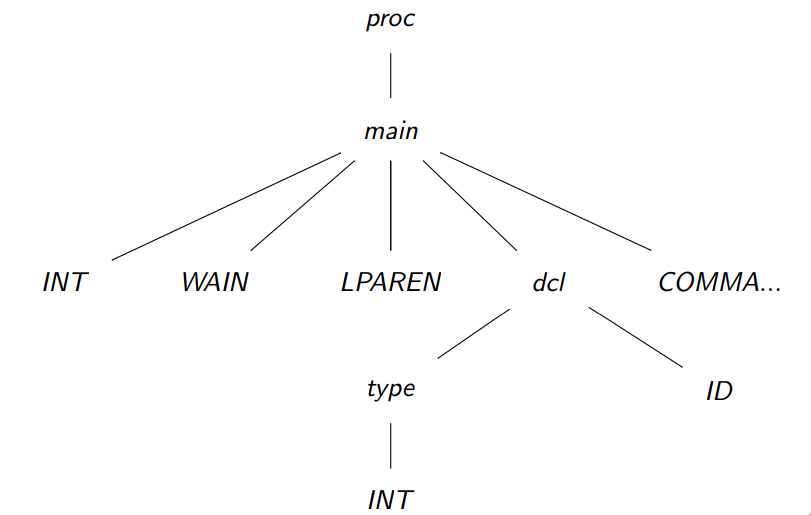
\includegraphics[scale=0.5]{parse_tree.png}
    \item In code, you could use a \emph{very} simple tree object:
        \begin{lstlisting}[mathescape, numbers=none, breaklines=true]
    class Tree {
        public:
            string rule;
            vector <string> tokens;
            vector <Tree> children;
    };
        \end{lstlisting}
    \item How could we determine multiple/missing declaration errors?  Use a symbol table!
    \item We don't have to pass through the file twice - this is because we cannot use variables before they are declared!
    \item We need to keep track of \emph{functions} and \emph{variables}!  
    \item Use a map that tracks functions (global) and a map for each function declaration if that is valid!
    \item You may need to keep a global variable that tracks which procedure we're in.
    \item For functions, we \emph{only} need to store the parameters, as WLP4 is limited to int type only for functions.
    \item We do need to be careful - we must ensure that the parameters passed in are the \emph{correct} parameters - we don't want int pointers if we want ints!
    \item Symbol tables should be a procedure name, pairs of signatures, and symbol tables.  This could be a \lstinline[mathescape]{map<string, pair<vector<string>, map<string, string>>>}
    \item Likewise, unlike rustcc, since this has support for pointers, we must keep track of those as well.  We have two types: ints and pointers to ints.  For type checking, upon delcaration, we add it to the symbol table.
    \item So for example, given the following code:
        \begin{lstlisting}[mathescape, numbers=none, breaklines=true]
    int f() {
        int *a = NULL;
        return 9;
    }

    int wain(int a, int b) {
        int x = 10;
        return x + a + b;
    }
        \end{lstlisting}
    this would return a symbol table with the two entries:
    \begin{itemize}
        \item \lstinline[mathescape]{f <>, <a ->, int*>}
        \item \lstinline[mathescape]{wain<int, int>}, and \lstinline[mathescape]{<a -> int, b -> int, x -> int>}
    \end{itemize}
    \item So, how do we actually catch a type error?
        \begin{itemize}
            \item First, we figure out the type of every epxression using type rules.
            \item Then, if none such rule exists or the types do not match a given rule, produce an error.
        \end{itemize} 
    \item We use inference rules from 245 - if an ID is declared with type $\tau$ then it has type int if there is a NUM, and int* if it there is a NULL.  That is, $\frac{<id.name, \tau> \in declarations}{id.name : \tau}$.
    \item $\frac{E: \tau}{(E) : \tau}$
    \item $\frac{E: int}{\&E: int*}$
    \item $\frac{E: int*}{*E: int}$
    \item $\frac{E: int}{new int [E]: int*}$
    \item $\frac{E_1: int, E_2: int}{E_1 +-/*\% E_2: int}$
    \item $\frac{E_1: int*, E_2: int}{E_1 +- E_2: int*}$
    \item $\frac{E_1: int, E_2: int*}{E_1 +- E_2: int*}$
    \item $\frac{E_1: int*, E_2: int*}{E_1 - E_2: int*}$
\end{itemize}

\end{document}

